Visualization tools are an important aspect of network analysis.  
For example, after completing a sensor placement optimization, it is important to 
understand how the physical location of the sensors relates to the underlying
structure of the water distribution network. The \code{visualization} subcommand 
overlays graphical layers on a water distribution network
and creates a HyperText markup language (HTML) file 
with scalar vector graphics that can be opened in a Web browser.  
The HTML file provides an interactive visualization of the results
from which images can be saved for later use via a screen capture (saved as a JPEG, PNG). 
%The graphic can be used in presentations and documents by
%saving the screen image as a graphics file (e.g., PNG, JPEG). 
After the HTML file is opened in a Web browser, the user has the ability to
(1) scroll over node and link elements to identify the respective EPANET ID, 
(2) scroll over the legend to isolate a specific layer, 
(3) move the legend and 
(4) zoom or pan the screen to change the size and location of the network.

The \code{visualization} subcommand includes an extensive number of graphic options within the 
configuration file.
To format the appearance of the network model, the user can define the color, size 
and opacity for the network elements (e.g., junctions, reservoirs, tanks, pipes, 
pumps and valves). The user can also decide 
which network elements to include in the legend.
Multiple node and link layers can then overlay the network model.  
The order of those layers is defined by the user.
For each layer, the user can select the layer shape (for node layers) along with the 
color, size and opacity. The color, size and opacity can be defined as a 
constant or can be set as a function of the layers value.
These options can be set independently for the layers fill and line.
Each layer is assigned a label to be used in the legend.
Other options include the screen size and background color, and the legend location
and background color.

Several WST subcommands automatically run the \code{visualization} subcommand 
upon completion to generates graphical representation of the results. These include 
\code{sp}, \code{flushing}, \code{booster\_msx}, \code{booster\_mip}, \code{inversion} and \code{grabsample}.
The graphic can be modified by editing the \code{visualization} 
configuration file, which is also automatically generated, and rerunning the \code{visualization} subcommand.
A flowchart representation of the \code{visualization} subcommand is shown in Figure \ref{fig:visualization-flowchart}. 
The utility network model is defined by an EPANET 2.00.12 compatible network model (INP format). 
Graphic options are supplied through the \code{visualization} WST configuration file.

\begin{figure}[h]
  \centering
  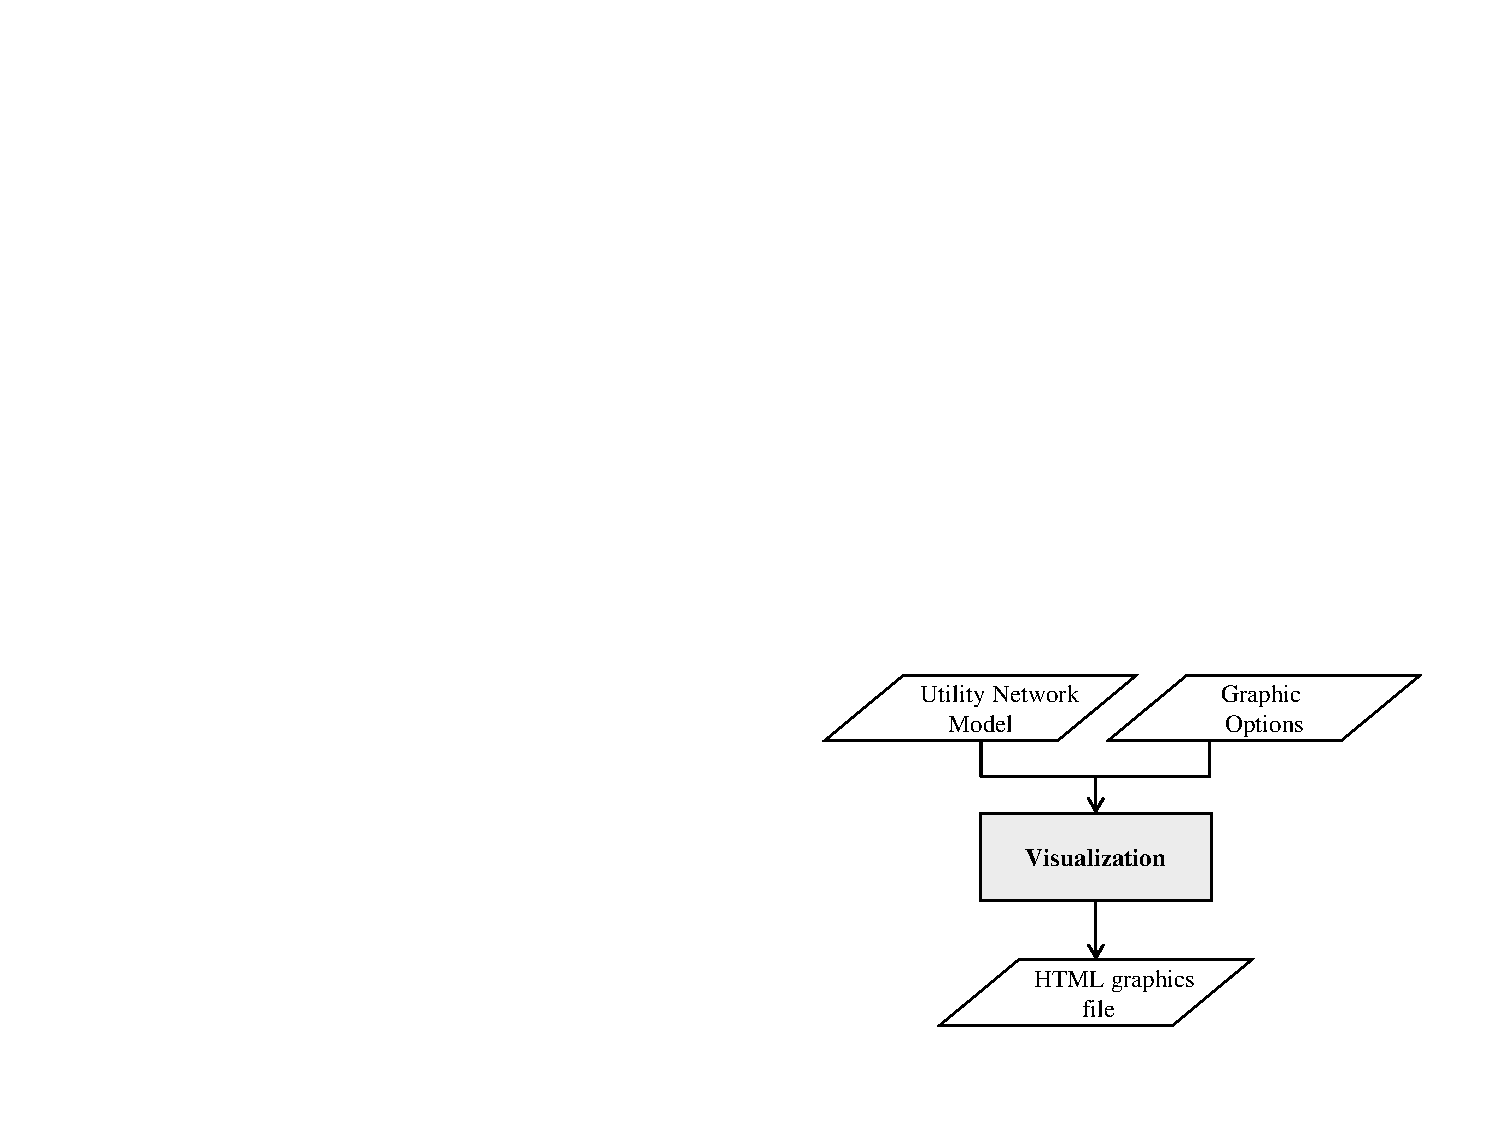
\includegraphics[scale=0.80]{graphics/visualization_flowchart.pdf}
  \caption{Visualization flowchart.}
  \label{fig:visualization-flowchart}
\end{figure}

\section{Color and Shape Options}
The color of a network element is specified using a six character hexadecimal (HEX) color code or using a 
predefined color name. HEX color codes can be found at various website, 
including \url{http://www.color-hex.com/color-wheel/}, and can be used to create 
any color between black (\#000000) and white (\#FFFFFF).
The following predefined colors can also be used in the the \code{visualization} 
subcommand.
\begin{unknownListing}
  Name    RGB           HEX
============================================
  red     [225,0,0]     \#FF0000 
  orange  [225,165,0]   \#FFA500
  yellow  [225,225,0]   \#FFFF00  
  green   [0,128,0]     \#008000
  blue    [0,0,225]     \#0000FF
  purple  [128,0,128]   \#800080
  black   [0,0,0]       \#000000
  white   [225,225,225] \#FFFFFF
  lime    [0,225,0]     \#00FF00
  navy    [0,0,128]     \#000080
  aqua    [0,225,225]   \#00FFFF
  teal    [0,128,128]   \#008080
  olive   [128,128,0]   \#808000
  maroon  [128,0,0]     \#800000
  fuchsia [225,0,225]   \#FF00FF
  silver  [192,192,192] \#C0C0C0
  gray    [128,128,128] \#808080
\end{unknownListing}

The shape of a network element is specified using one of the following predefined shapes, using 
either the long or short name.
\begin{unknownListing}
  Long Name    Short Name   
===========================
  circle        o
  square        s
  triangle      t
  diamond       d
  plus          +
  x		x
\end{unknownListing}

\section{Data from YAML Files}
Within the \code{visualization} WST configuration file, layers can be 
defined by 
(1) directly including the network element values, or
(2) referencing data in an external YAML file.

The following subset of a \code{visualization} WST configuration file 
demonstrates how element values are directly included in the layers block. 
\begin{unknownListing}
layers:
  locations: ['115', '101', '171']   
  file: null
\end{unknownListing}

The same data can be stored in an external YAML file and referenced in the 
\code{visualization} WST configuration file, as shown below. 
\begin{unknownListing}
layers:
  locations: '["flushing"]["nodes"][i]'
  file: data.yml
\end{unknownListing}
In this example, the referenced file, data.yml, contains the following information. 
\begin{unknownListing}
flushing:
  nodes: ['115', '101', '171']   
\end{unknownListing}

The WST subcommands (e.g., \code{sp}, \code{flushing}) that 
automatically run the \code{visualization} subcommand 
upon completion read data from external YAML files.

\section{\code{visualization} Subcommand}

The \code{visualization} subcommand is executed using the following command line:
\begin{unknownListing}
wst visualization <configfile> 
\end{unknownListing}
where \code{configfile} is a WST configuration file in the YAML format.  

The \code{---help} option prints information about this subcommand, such as usage,
arguments and a brief description:

\begin{unknownListing}
wst visualization --help
\end{unknownListing}

\subsection{Configuration File}

The \code{visualization} subcommand generates a template configuration file using the following command line:

\begin{unknownListing}
wst visualization --template <configfile>
\end{unknownListing}

The \code{visualization} WST template configuration file is shown in Figure \ref{fig:visualization_template}. 
Brief descriptions of the options are included in the template after the \# sign.  

\begin{figure}[H]
  \unknownInputListing{examples/visualization_config.yml}{}{1}{64}
  \caption{The \code{visualization} configuration template file.}
  \label{fig:visualization_template}
\end{figure}
  
\subsection{Configuration Options}

Full descriptions of the WST configuration options used by the \code{visualization} subcommand are listed below.
\begin{description}[topsep=0pt,parsep=0.5em,itemsep=-0.4em]
  \item[{network}]\hfill
  \begin{description}[topsep=0pt,parsep=0.5em,itemsep=-0.4em]
    \item[{epanet file}]\hfill
\\ The name of the EPANET 2.00.12 input (INP) file that defines the water distribution
                network model.
                
                Required input.
  \end{description}
  \item[{visualization}]\hfill
  \begin{description}[topsep=0pt,parsep=0.5em,itemsep=-0.4em]
    \item[{screen}]\hfill
    \begin{description}[topsep=0pt,parsep=0.5em,itemsep=-0.4em]
      \item[{color}]\hfill
\\The screen background color defined using a HEX color code or predefined color name.
                
                Optional input, default = white
      \item[{size}]\hfill
\\The screen size [width, height] in pixels.
                
                Optional input, default = [1000,600]
    \end{description}
    \item[{legend}]\hfill
    \begin{description}[topsep=0pt,parsep=0.5em,itemsep=-0.4em]
      \item[{color}]\hfill
\\The legend background color defined using a HEX color code or predefined color name.
                
                Optional input, default = white
      \item[{scale}]\hfill
\\The legend text size multiplier, real number.
                
                Optional input, default = 1.0
      \item[{location}]\hfill
\\The legend location [left, top] in pixels.
                
                Optional input, default = [10,10] (upper left)
    \end{description}
    \item[{nodes}]\hfill
    \begin{description}[topsep=0pt,parsep=0.5em,itemsep=-0.4em]
      \item[{color}]\hfill
\\The node color defined using HEX color code or predefined color name.
                The color will apply to junctions, reservoirs and tanks. If the 
                color is left blank, then junctions are black, reservoirs are 
                blue and tanks are green.
                
                Optional input, default = None
      \item[{size}]\hfill
\\The node size, real number.
                
                Optional input.
      \item[{opacity}]\hfill
\\The node opacity, real number between 0.0 (transparent) and 1.0 (opaque).
                
                Optional input, default = 0.6
    \end{description}
    \item[{links}]\hfill
    \begin{description}[topsep=0pt,parsep=0.5em,itemsep=-0.4em]
      \item[{color}]\hfill
\\The link color defined using HEX color code or predefined color name.
                The color will apply to pipes, pumps and valves. If the 
                color is left blank, then pipes are black, pumps are 
                yellow and valves are turquoise.
                
                Optional input, default = None
      \item[{size}]\hfill
\\The link size, real number.
                
                Optional input.
      \item[{opacity}]\hfill
\\The link opacity, real number between 0.0 (transparent) and 1.0 (opaque).
                
                Optional input, default = 0.6
    \end{description}
    \item[{layers}]\hfill
    \begin{description}[topsep=0pt,parsep=0.5em,itemsep=-0.4em]
      \item[{label}]\hfill
\\The layer label used in the legend. 
                
                Optional input, default = None
      \item[{locations}]\hfill
\\
                The data locations to plot over the network. Locations are specified
                using a list of EPANET IDs.
                
                Required input unless an external file is specified.
      \item[{file}]\hfill
\\The name of an external file that contains data to be used in the visualization.
                The file is in YAML format. 
                
                Required input unless 'locations' are specified.  
                Data from a file overrides data specified in 'locations'
      \item[{location type}]\hfill
\\The location type is used to indicate if the EPANET ID is of type 'node' 
                (junction, reservoir, tank) or 'link' (pipe, pump, valve).
                
                Optional input. If left blank, node is tested before link
      \item[{shape}]\hfill
\\The marker shape, used only for node type layers. The shape can
                be a single string, or a list of strings which is the same 
                length as the location data.
                
				Optional input, only used for node type layers, default = circle
      \item[{fill}]\hfill
      \begin{description}[topsep=0pt,parsep=0.5em,itemsep=-0.4em]
        \item[{color}]\hfill
\\The fill color defined using HEX color code or predefined color name.
                
                Optional input, default = None
        \item[{size}]\hfill
\\The fill size, real number.
                
                Optional input.
        \item[{opacity}]\hfill
\\The fill opacity, real number between 0.0 (transparent) and 1.0 (opaque).
                
                Optional input, default = 0.6
        \item[{color range}]\hfill
\\The fill color range used to scale line data.
                
                Optional input, default = [data min, data max]
        \item[{size range}]\hfill
\\The fill size range used to scale line data.
                
                Optional input, default = [data min, data max]
        \item[{opacity range}]\hfill
\\The fill opacity range used to scale line data.
                
                Optional input, default = [data min, data max]
      \end{description}
      \item[{line}]\hfill
      \begin{description}[topsep=0pt,parsep=0.5em,itemsep=-0.4em]
        \item[{color}]\hfill
\\The line color defined using HEX color code or predefined color name.
                
                Optional input, default = None
        \item[{size}]\hfill
\\The line size, real number.
                
                Optional input.
        \item[{opacity}]\hfill
\\The fill opacity, real number between 0.0 (transparent) and 1.0 (opaque).
                
                Optional input, default = 0.6
        \item[{color range}]\hfill
\\The line color range used to scale line data.
                
                Optional input, default = [data min, data max]
        \item[{size range}]\hfill
\\The line size range used to scale line data.
                
                Optional input, default = [data min, data max]
        \item[{opacity range}]\hfill
\\The line opacity range used to scale line data.
                
                Optional input, default = [data min, data max]
      \end{description}
    \end{description}
  \end{description}
  \item[{configure}]\hfill
  \begin{description}[topsep=0pt,parsep=0.5em,itemsep=-0.4em]
    \item[{output prefix}]\hfill
\\The prefix used for all output files.
                
                Required input.
    \item[{output directory}]\hfill
      \\The output directory to store the results.
    \item[{debug}]\hfill
\\The debugging level (0 or 1) that indicates the amount of debugging 
                information printed to the screen, log file and output yml file. 
                
                Optional input, default = 0 (lowest level).
  \end{description}
\end{description}


For additional control over the way that junctions, reservoir, tanks, pipes, pumps and valves are
displayed, the following YAML blocks can be added to the visualization configuration block.
The color, size and opacity of each element can be changed; and the element can
be added to the legend. These options will override the node and link blocks.
\begin{unknownListing}
  junctions:
    color: red  
    size: 5.0
    opacity: 0.5
  reservoirs:
    color: orange
    size: 12.0
    opacity: 1
  tanks:
    color: yellow
    size: 12.0
    opacity: 1
  pipes:
    color: green
    size: 3.0
    opacity: 0.5
  pumps:
    color: blue
    size: 3.0
    opacity: 1
  valves:
    color: purple
    size: 3.0
    opacity: 0.7
\end{unknownListing}
\subsection{Subcommand Output}

The \code{visualization} subcommand creates a HTML file 
named <output prefix>visualization\_output.html
that contains scalar vector graphics that can be opened in a Web browser.  
Two other files are created: 
(1) an output YAML file named <output prefix>visualization\_output.yml
that includes run date and CPU time, and 
(2) a log file named <output prefix>visualization\_output.log
that includes basic debugging information.

\section{Visualization Examples}\label{visualization_example}

An EPANET 2.00.12 network model input file (INP format) and a configuration file, which contain the
graphics options, are required to run the \code{visualization} subcommand.  
Several examples for visualization are given below.

\subsection{Example 1}

The first example customizes the color, size and opacity of the network
elements (junctions, reservoirs, tanks, pipes and pumps). The reservoir and 
tank colors are specified using HEX color codes. Additionally, the graphic
highlights five pipes and uses their diameter to scale the pipe width. 
All the data is supplied in the configuration file.  
The configuration file, visualization\_ex1.yml, for this example is shown in Figure \ref{fig:visualization_ex1}.  

\begin{figure}[h]
  \unknownInputListing{../../examples/visualization_ex1.yml}{}{1}{46}
  \caption{The \code{visualization} configuration file for example 1.}
  \label{fig:visualization_ex1}
\end{figure}

The example can be executed using the following command line:

\begin{unknownListing}
wst visualization visualization_ex1.yml
\end{unknownListing}

The resulting graphic is shown in Figure \ref{fig:visualization_graphic_ex1}.

\begin{figure}[h]
  \centering
  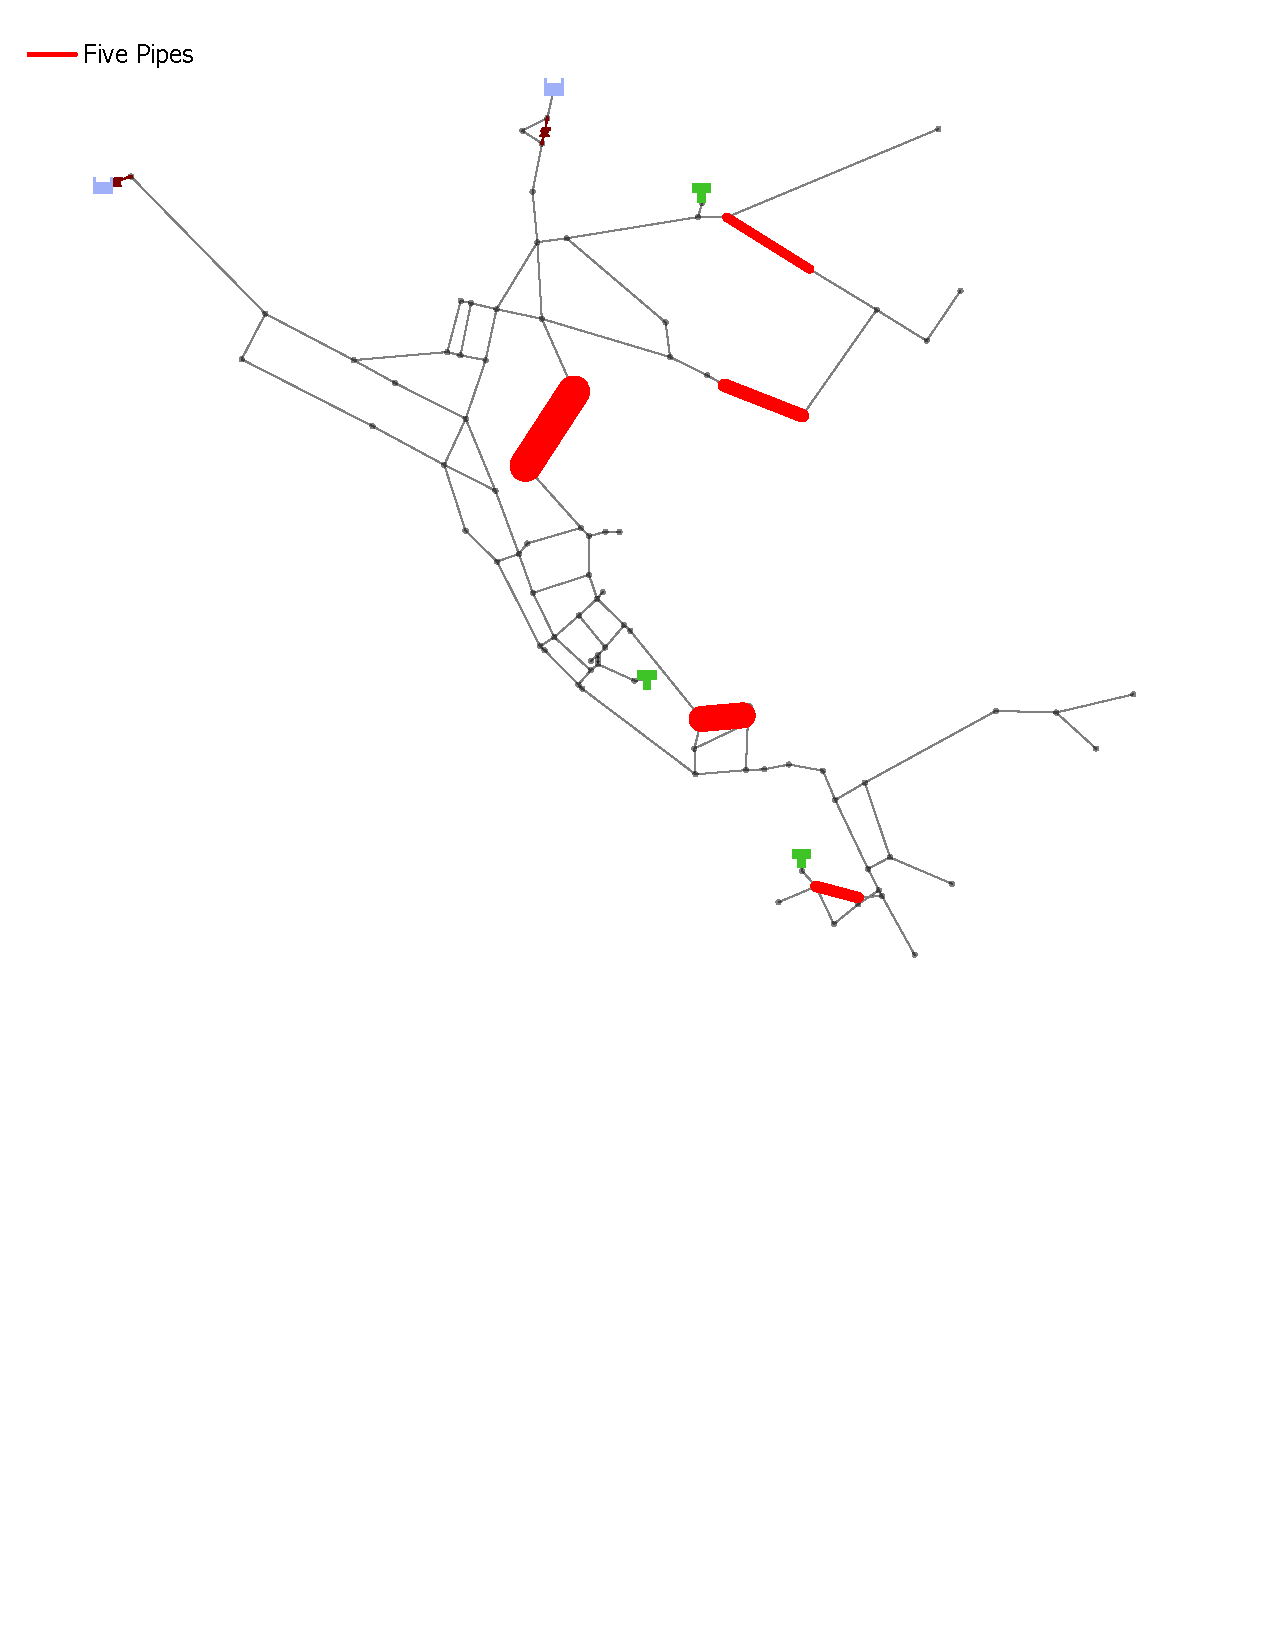
\includegraphics[scale=0.80]{examples/visualization_ex1.pdf}
  \caption{Graphic from \code{visualization} example 1.}
  \label{fig:visualization_graphic_ex1}
\end{figure}

\FloatBarrier 
\subsection{Example 2}

The second example uses an external data file to define locations and values to
be used in the network graphic.
The configuration file, visualization\_ex2.yml, for this example is shown in Figure \ref{fig:visualization_ex2}.  
The location file used in this example is shown in Figure \ref{fig:visualization_locations_ex2}. 
This example uses the pipe length to scale the size and opacity of the links and 
the base demand to scale the color and size of the nodes. This graphic 
shows that link 329 is very long compared to the other 30-inch diameter pipes and 
that node 109 has the largest base demand. The size range option in the configuration file   
is used to automatically scale the size and opacity of each layer. For example, 
the link length ranges from 1 to 45,500, but is scaled to a size range of 5 to 20.   
\begin{figure}[h]
  \unknownInputListing{../../examples/visualization_ex2.yml}{}{1}{38}
  \caption{The \code{visualization} configuration file for example 2.}
  \label{fig:visualization_ex2}
\end{figure}

\begin{figure}[h]
  \unknownInputListing{../../examples/Net3/Net3_locations.yml}{}{1}{5}
  \caption{The location file used in \code{visualization} example 2.}
  \label{fig:visualization_locations_ex2}
\end{figure}

The example can be executed using the following command line:

\begin{unknownListing}
wst visualization visualization_ex2.yml
\end{unknownListing}

The resulting graphic is shown in Figure \ref{fig:visualization_graphic_ex2}.

\begin{figure}[h]
  \centering
  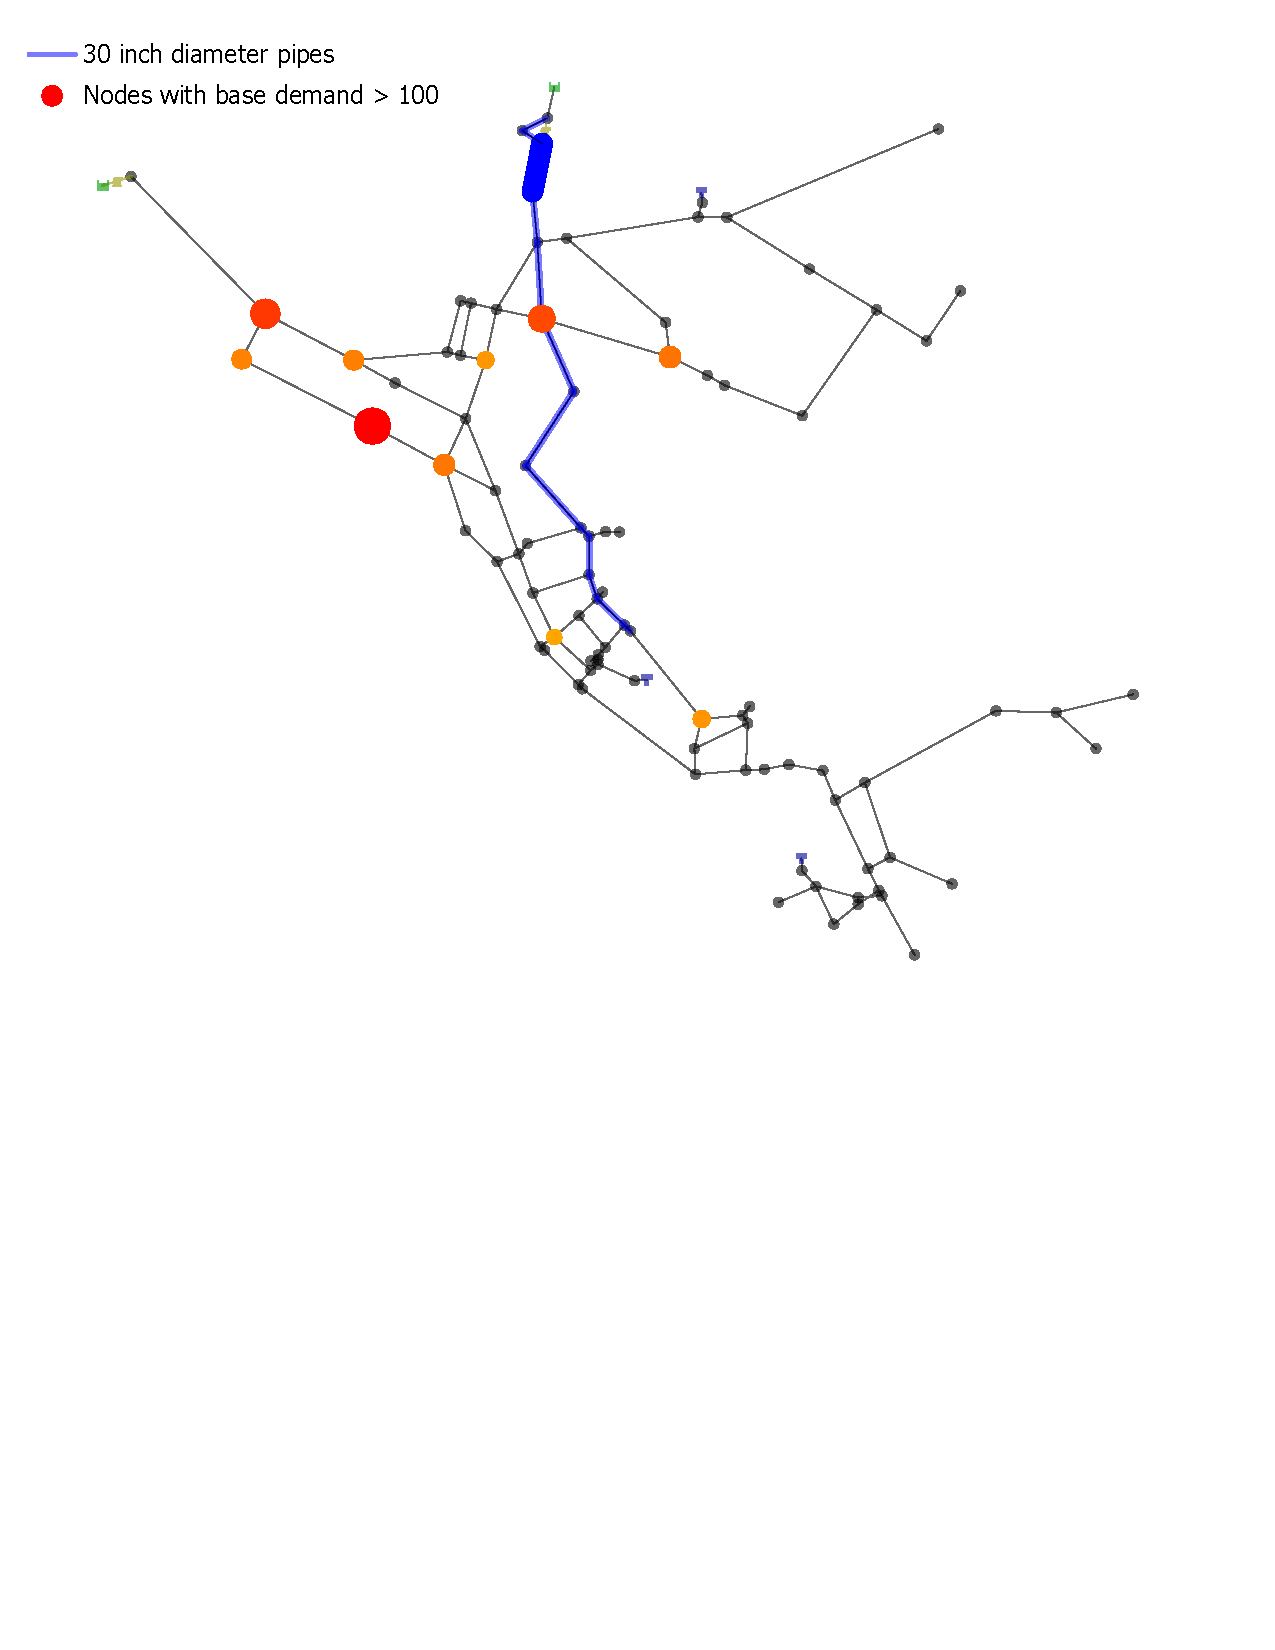
\includegraphics[scale=0.80]{examples/visualization_ex2.pdf}
  \caption{Graphic from \code{visualization} example 2.}
  \label{fig:visualization_graphic_ex2}
\end{figure}

